\hypertarget{czas_8cpp}{\section{Dokumentacja pliku /home/karolina/\-Pulpit/pamsi6/prj/src/czas.cpp}
\label{czas_8cpp}\index{/home/karolina/\-Pulpit/pamsi6/prj/src/czas.\-cpp@{/home/karolina/\-Pulpit/pamsi6/prj/src/czas.\-cpp}}
}


Definicja metody Start.  


{\ttfamily \#include \char`\"{}czas.\-hh\char`\"{}}\\*
Wykres zależności załączania dla czas.\-cpp\-:\nopagebreak
\begin{figure}[H]
\begin{center}
\leavevmode
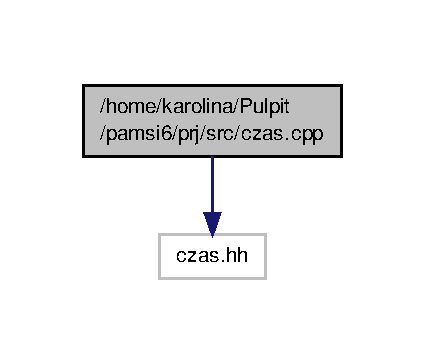
\includegraphics[width=204pt]{czas_8cpp__incl}
\end{center}
\end{figure}


\subsection{Opis szczegółowy}
Definicja metody Wynik.

Definicja metody Koniec.

Metoda, ktora wlacza zegar.

Metoda, ktora powoduje zatrzymanie zegara i liczy czas dzialania algorytmu.

Metoda, ktora wyswietla wynik. 

Definicja w pliku \hyperlink{czas_8cpp_source}{czas.\-cpp}.

